\documentclass{beamer}
\usepackage[utf8]{inputenc}
\usepackage{multicol}
\usetheme{cern}
\usepackage{wrapfig}

%The CERN logo is legally protected. Please visit http://cern.ch/copyright for information on the terms of use of CERN content, including the CERN logo.

% The optional `\author` command defines the author and is displayed in the slide produced by the `\titlepage` command.
\author{Hannah Short (CERN), Sebastian Lopienski (CERN)}

% The optional `\title` command defines the title and is displayed in the slide produced by the `\titlepage` command.
\title{Practical Security and Cryptography}

% The optional `\subtitle` command will add a smaller title below the main one, and will not be displayed in any of the slides' footer.
\subtitle{CODATA School}

% The optional `\date` command will display a custom free text date on the all of the slides' footer. If omitted today's date will be used.
%\date{Monday, 1st January 2018}

\begin{document}

\frontcover

% The optional `\titlepage` command will create a slide with the presentation's title, subtitle and author.
\frame{\titlepage}

\begin{frame}{Lecturers}
These slides have been compiled by members of the CERN Computer Security Team based at CERN, the European Organisation for Nuclear Research.
\begin{center}
\begin{tabular}{ c c  }
 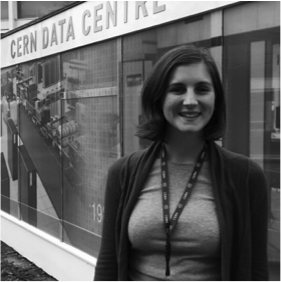
\includegraphics[width=0.2\linewidth]{lecturer1.png} & 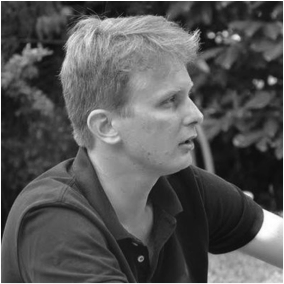
\includegraphics[width=0.2\linewidth]{Lecturer2.png}  \\ 
 Hannah Short & Sebastian Lopienski  \\  
\end{tabular}
\end{center}
\end{frame}

% The optional `\tableofcontents` command will automatically create a table of contents based om the sections.
\frame{\tableofcontents}

\begin{frame}{Course Objectives}
	\begin{itemize}
		\item Understand the key concepts of cryptography
		\item Learn to identify good practices in web security
	\end{itemize}
\textbf{Note:} \newline
\textit{}{If the slide title is in {\color{red}red}, the slide is considered an advanced topic}
\end{frame}

\section{Introduction to Encryption}
\frame{\sectionpage}

\begin{frame}{}
\begin{center}
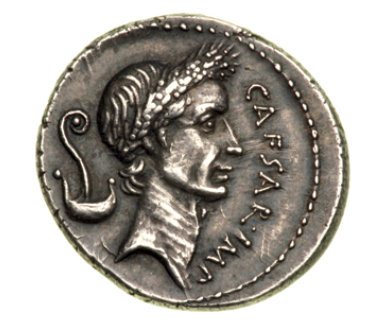
\includegraphics[width=0.7\linewidth]{coin.png}
\end{center}
\end{frame}

\begin{frame}{Caesar Cipher}
If he had anything confidential to say, he wrote it in cipher, that is, by exchanging the order of the letters of the alphabet, that not a word could be made out.  If anyone wishes to decipher these, and get at their meaning, he must substitute the fourth letter of the alphabet, namely D, for A, and so with the others - \textit{Suetonius, Life of Julius Caesar}
\end{frame}

\begin{frame}{Caesar Cipher}
\begin{center}
Pxkqx Zixrp fp zljfkd ql qltk \newline
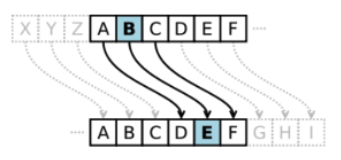
\includegraphics[width=0.7\linewidth]{caesar-cipher.png}\newline
\end{center}
\end{frame}

\begin{frame}{Caesar Cipher}
\begin{center}
Pxkqx Zixrp fp zljfkd ql qltk \newline
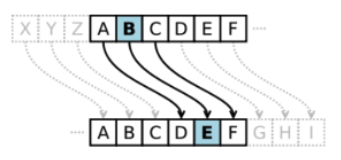
\includegraphics[width=0.7\linewidth]{caesar-cipher.png} \newline
Santa Claus is coming to town
\end{center}
\end{frame}

\begin{frame}{Caesar Cipher}
\begin{itemize}
\item Cipher = Caesar Cipher
\item Key = 3
\item Plaintext = Santa Claus is coming to town
\item Ciphertext =  Pxkqx Zixrp fp zljfkd ql qltk
\end{itemize}
What could be a weakness of this Cipher?
\end{frame}

\begin{frame}{Caesar Cipher}
\begin{itemize}
\item Only 26 keys
\item Easy to brute force
\item How can we improve on this?
\end{itemize}
\end{frame}

\begin{frame}{Monoalphabetic Substitution Cipher}
\begin{center}
ABCDEFGHIJKLMNOPQRSTUVWXYZ
BCEZUMPFRDJIYONGTXVLAHKQSW
\end{center}
\begin{itemize}
\item Cipher = Monoalphabetic Substitution Cipher
\item Key = BCEZUMPFRDJIYONGTXVLAHKQSW
\item Plaintext = Santa Claus is coming to town
\item Ciphertext =  Vbolb Eibav rv enyrop ln lnko
\end{itemize}
\end{frame}

\begin{frame}{Monoalphabetic Substitution Cipher}
 Number of possible keys = \( 26\times25\times ... \times2\times1\)
 \newline
\(26! = 403 291 461 126 605 635 584 000 000\)
\end{frame}

\begin{frame}{Monoalphabetic Substitution Cipher}
How could you crack it?
\begin{itemize}
\item In each language, some letters are more common than others
\item Could you use this to your advantage?
\end{itemize}
\end{frame}

\begin{frame}{Why Encryption?}
\begin{center}
	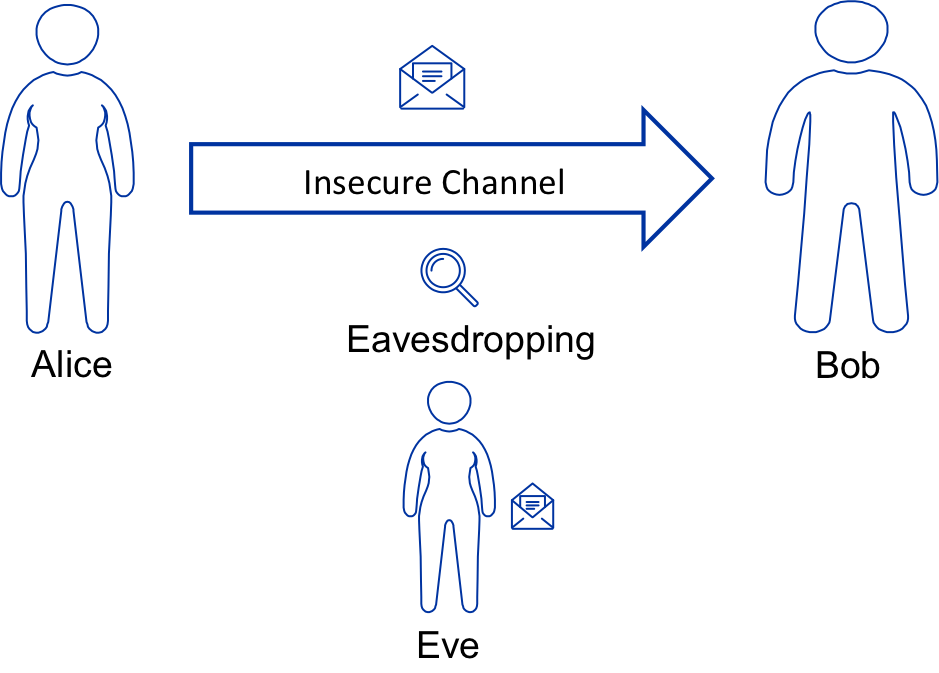
\includegraphics[width=0.7\linewidth]{insecure-channel.png}
\end{center}
\end{frame}

\begin{frame}{Why Encryption?}
What are the goals? 
\begin{itemize}
  \item \textbf{Confidentiality}: To prevent adversaries from viewing/accessing messages
  \item \textbf{Integrity}: To prevent adversaries from silently modifying messages
  \item \textbf{Authentication}: To prevent adversaries from impersonating an identity
  \item \textbf{Non-repudiation}: To prevent adversaries from denying an action
\end{itemize}
\end{frame}

\begin{frame}{Encryption in practice}
\begin{itemize}
\item There are several common, robust encryption algorithms available (e.g. AES and RSA) 
\item A good encryption algorithm relies on keeping the key secret, not the cipher algorithm itself!
\item Choose a well known, secure algorithm and keep the key secure (do not trust proprietary algorithms)
\item There are two main types; \textbf{Symmetric and Asymmetric} 
\end{itemize}
\end{frame}

\begin{frame}{Symmetric Encryption}
\begin{center}
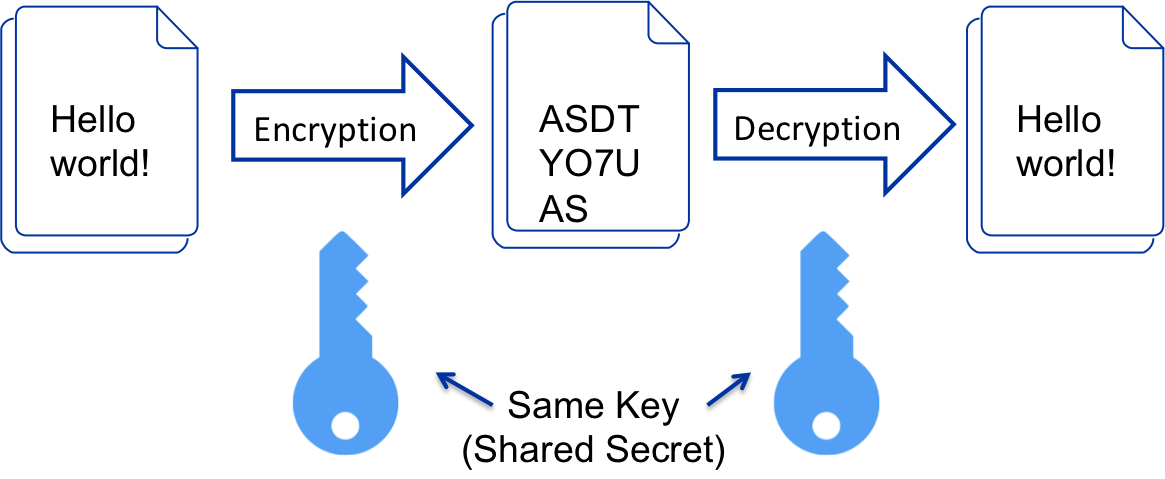
\includegraphics[width=0.8\linewidth]{symmetric-encryption.png}
\end{center}
\end{frame}

\begin{frame}{Asymmetric Encryption}
\begin{center}
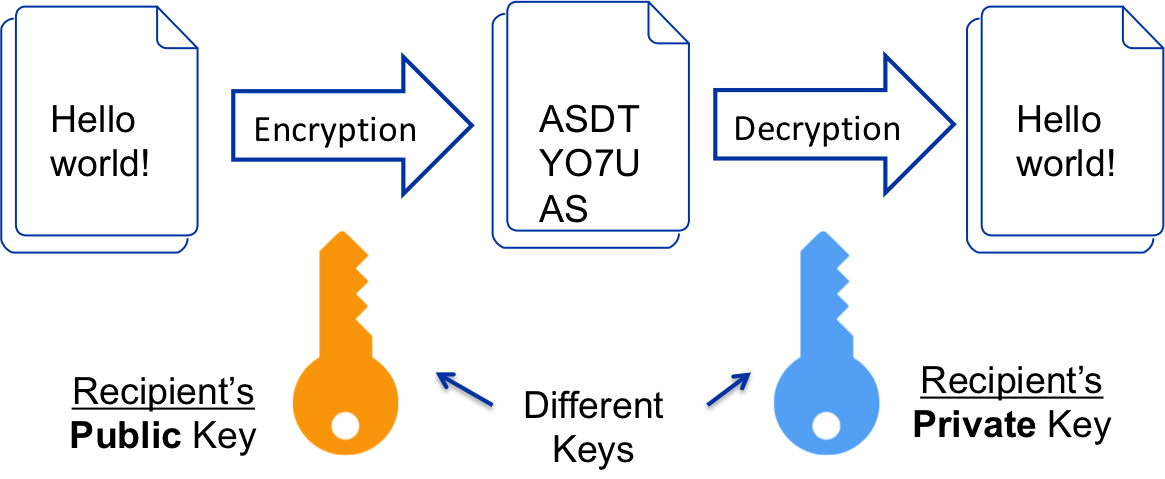
\includegraphics[width=0.8\linewidth]{asymmetric-encryption.png}
\end{center}
\end{frame}

\begin{frame}{Asymmetric Encryption}
\begin{center}
	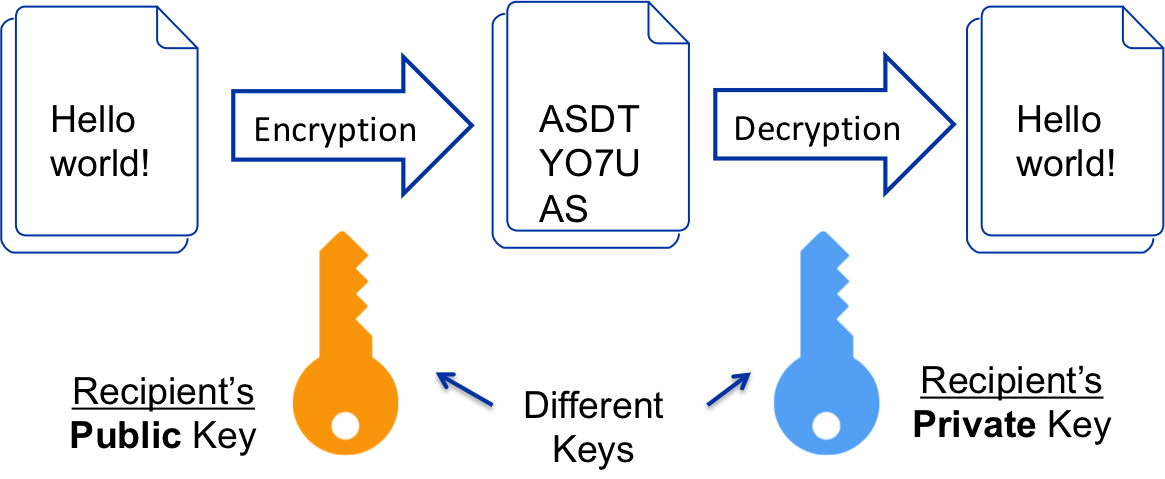
\includegraphics[width=0.45\linewidth]{asymmetric-encryption.png}
\end{center}
2 interchangeable (linked) keys
\begin{itemize}
  \item Public + Private 
  \item Mathematically difficult to compute one from the other 
  \item 1 for encryption and the other decryption
\end{itemize} 
\end{frame}

\begin{frame}{{\color{red}Asymmetric Encryption}}
\begin{itemize}
\item Relies on the fact that it is \textbf{easy} to multiply primes but hard to factorise their product
\item Consider the number 221... what are its factors?
\item Security is dependent on the status of computing technologies (it's secure now, but won't be in 100 years...)
\end{itemize}
\end{frame}

\begin{frame}{{\color{red}Asymmetric Enc. - Confidentiality}}
\begin{center}
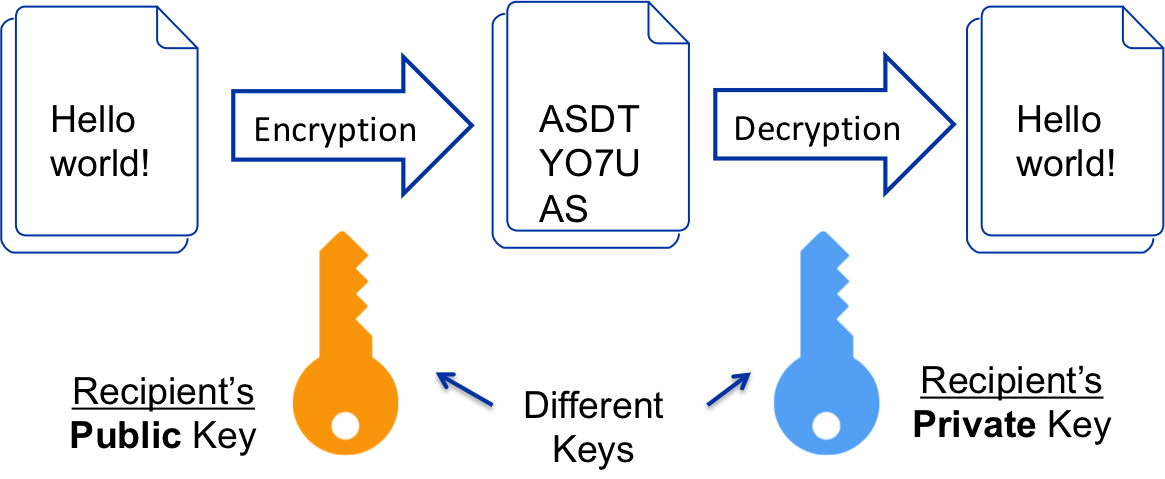
\includegraphics[width=0.9\linewidth]{asymmetric-encryption.png}
\end{center}
\end{frame}

\begin{frame}{{\color{red}Asymmetric Enc. - Authentication}}
\begin{center}
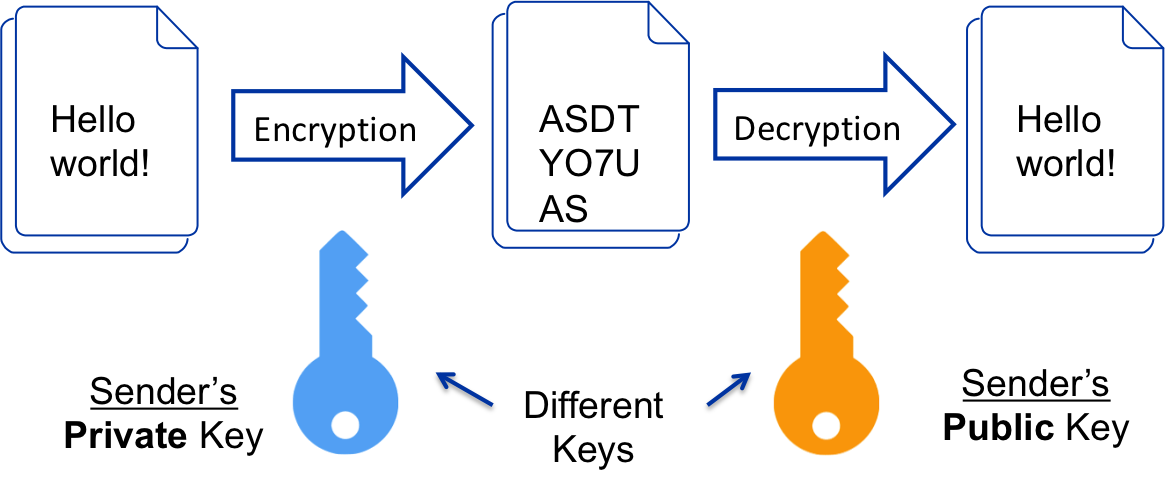
\includegraphics[width=0.9\linewidth]{asymmetric-authentication.png}
\end{center}
\end{frame}

\begin{frame}{Encryption - Summary}
\begin{itemize}
\item Encryption can be used for confidential, authenticated communication 
\item Symmetric and Asymmetric Ciphers have evolved over time
\end{itemize}
\end{frame}

\section{Hash Functions}
\frame{\sectionpage}

\begin{frame}{Hash Functions}
A hash function is any function that can be used to map data of arbitrary size to data of a fixed size.
\end{frame}

\begin{frame}{Hash Functions}
How can we make something of a fixed length? 
\begin{itemize}
\item We want the input (however long) to turn into one of a smaller range of possible outputs
\item Consider a registration process where attendees pick up their badges based on the first letter of surname... 
\begin{center}
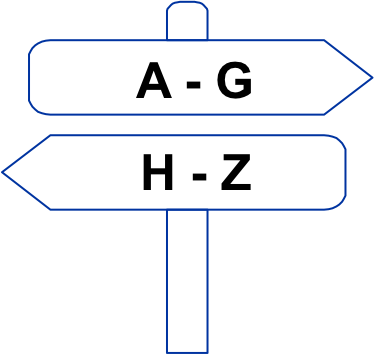
\includegraphics[width=0.3\linewidth]{surname-sort.png}
\end{center}
\end{itemize}
\end{frame}

\begin{frame}{Hash Functions}
E.g. \textit{``Today is gonna be the day that they're gonna throw it back to you. By now you should've somehow realized what you gotta do. I don't believe that anybody feels the way I do, about you now"} 
becomes \textbf{0283bf5eb0c60213a99f011a89300179} using the MD5 hashing algorithm
\newline
\url{https://passwordsgenerator.net/md5-hash-generator/}
\end{frame}

\begin{frame}{Hash Functions}
What is a *good* hash function? For \(h = hash(m)\)
\begin{itemize}
\item Difficult to find any message \(m\) with a given hash value \(h\)
\item Difficult to find 2 messages \(m1\), \(m2\) such that: \(hash(m1) = hash(m2)\)
\end{itemize}
\begin{center}
	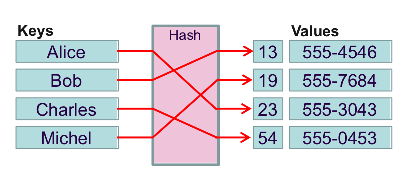
\includegraphics[width=0.5\linewidth]{hash.png}
\end{center}
\end{frame}

\begin{frame}{{\color{red}Hash Functions - a Use Case}}
\begin{center}
	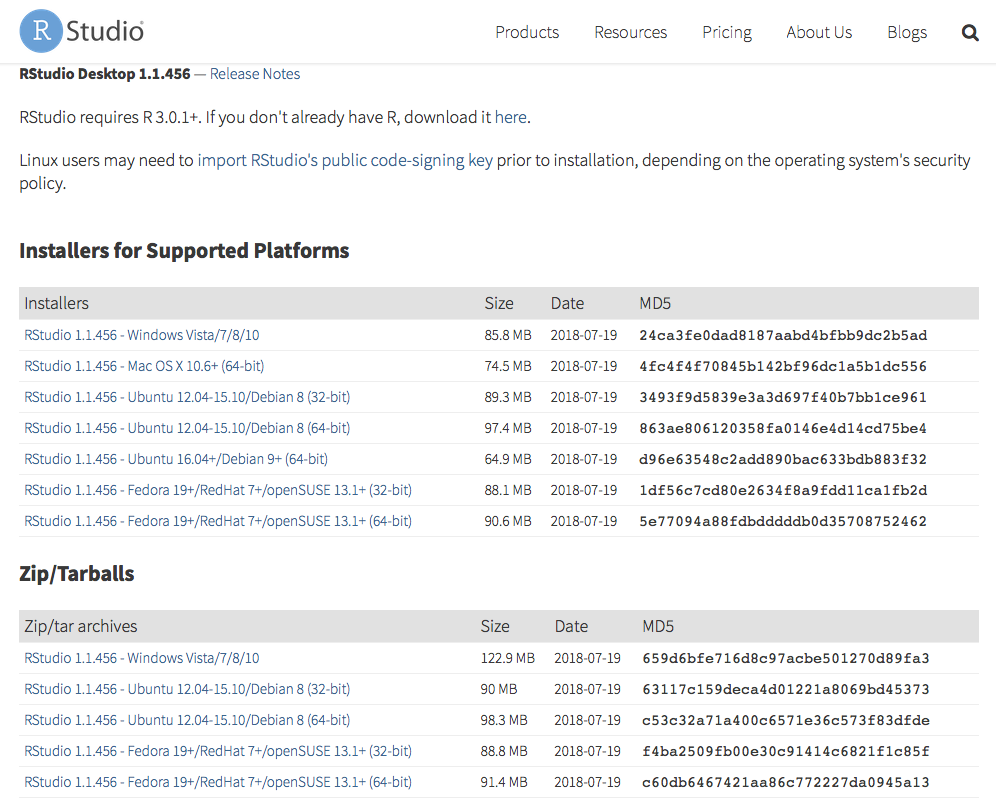
\includegraphics[width=0.65\linewidth]{r-studio.png}
    \newline
	{\footnotesize \url{https://www.rstudio.com/products/rstudio/download/} }
\end{center}
\end{frame}

\begin{frame}{Hash Functions - another Use Case}
\begin{itemize}
\item Instead of storing passwords, secure services store their hashes!
\item What would happen if the database is compromised?
\end{itemize}
\end{frame}

\begin{frame}{Hash Functions - another Use Case}
\begin{itemize}
\item Instead of storing passwords, secure services store their hashes!
\item What would happen if the database is compromised?
\begin{itemize}
\item \textbf{Dictionary attacks still valid}
\item This can be avoided by "salting" passwords, the system adds digits before hashing
\end{itemize}
\end{itemize}
\end{frame}

\begin{frame}{Checksums}
You may also hear the term "\textbf{Checksum}". The concept is the same but checksums are used specifically to validate the integrity data. 
\begin{center}
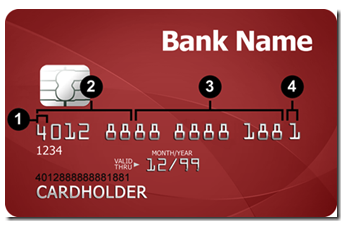
\includegraphics[width=0.45\linewidth]{credit-card.png} \newline
{\footnotesize The last digit is a checksum! \url{https://www.codeproject.com/Tips/515367/Validate-credit-card-number-with-Mod-algorithm} \par}
\end{center}
\end{frame}

\begin{frame}{Hash Functions - Summary}
\begin{itemize}
\item Hash functions transform arbitrary data to a fixed size in a deterministic (repeatable) way
\item There are multiple applications, e.g. file integrity \& password storage
\end{itemize}
\end{frame}

\section{Certificates}
\frame{\sectionpage}

\begin{frame}
\begin{center}
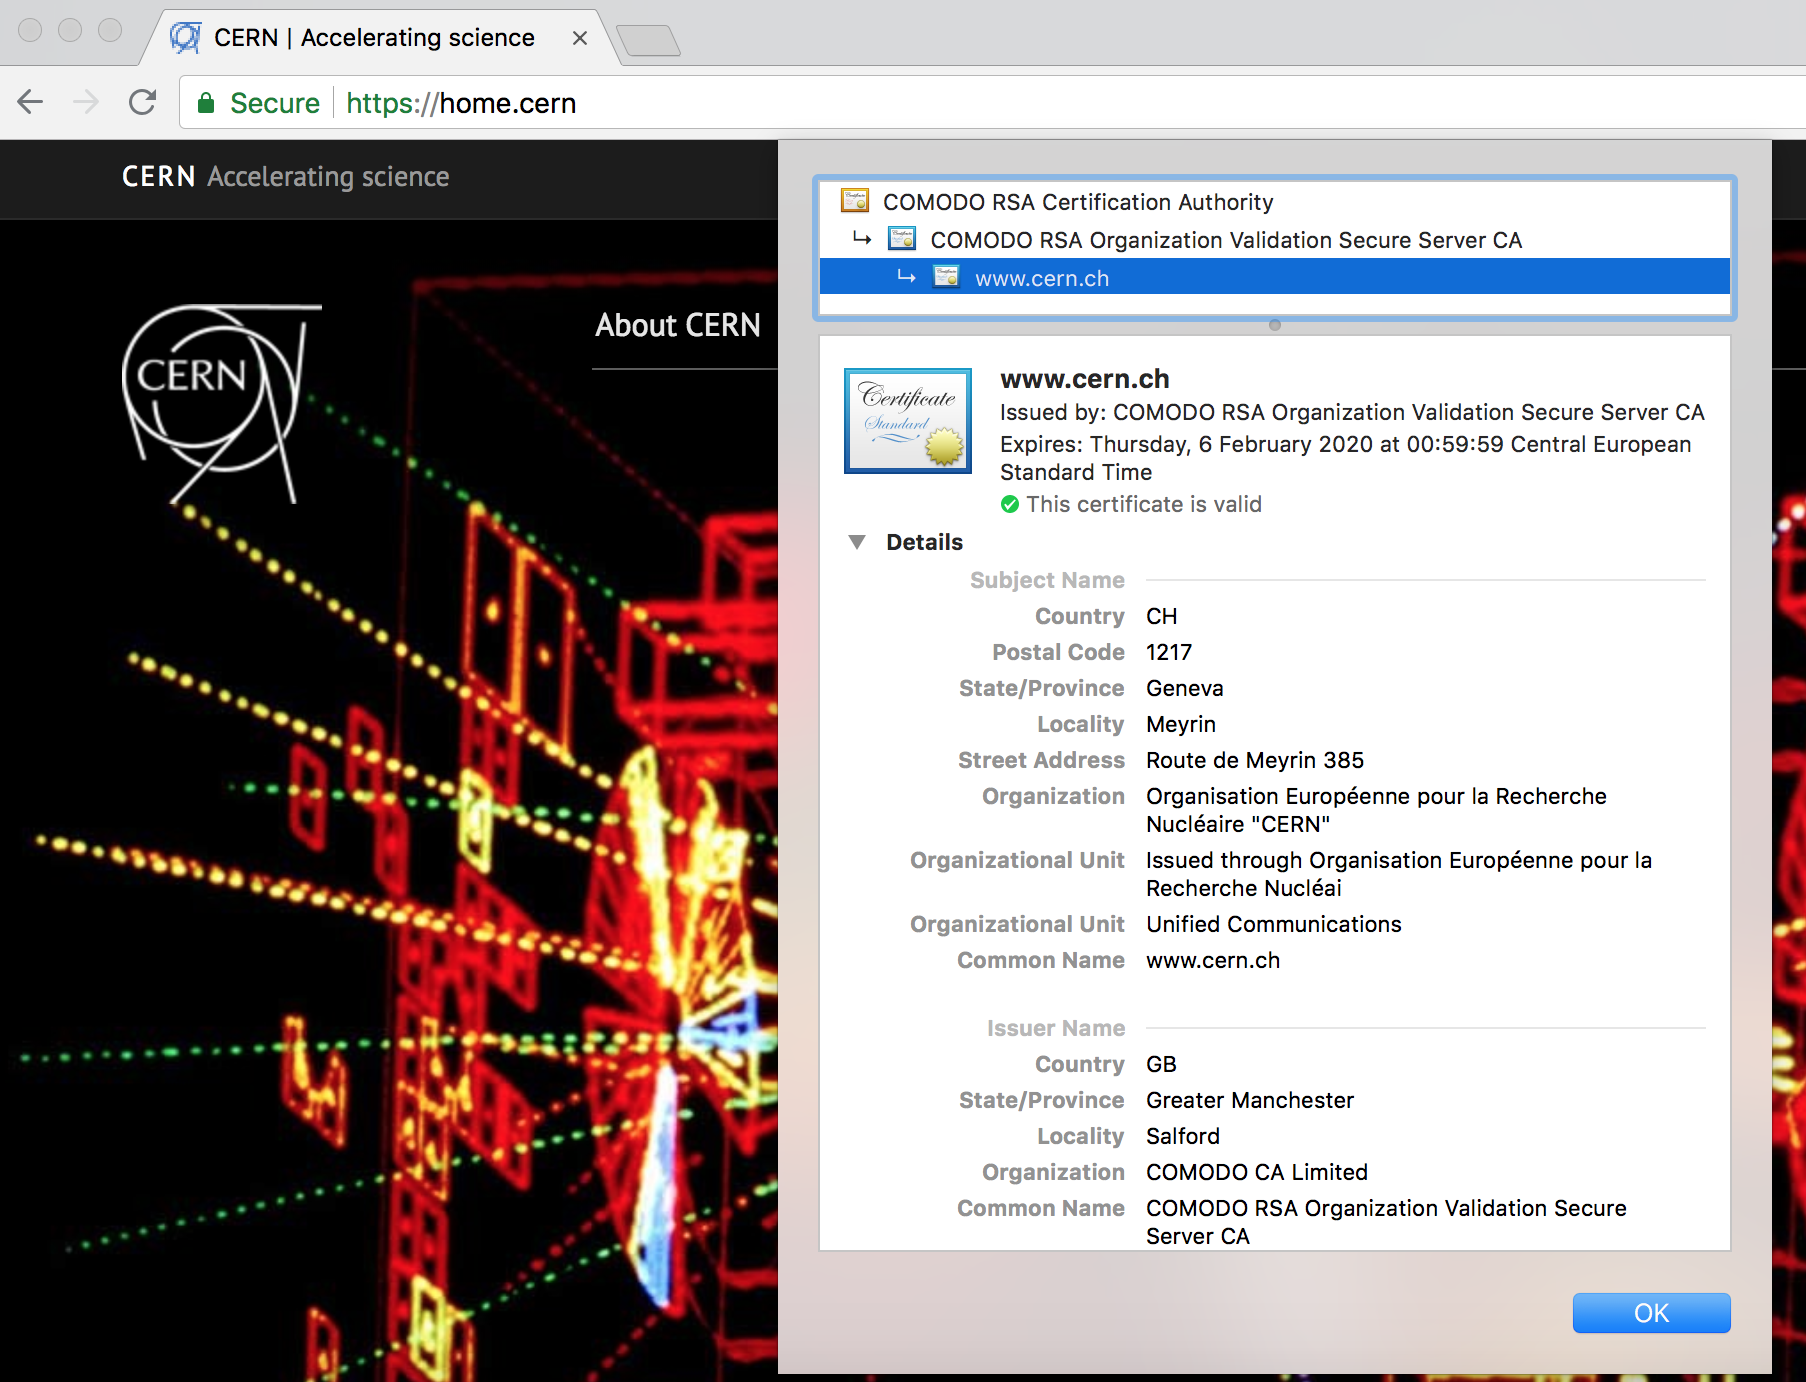
\includegraphics[width=0.9\linewidth]{cern-certificate.png}
\end{center}
\end{frame}

\begin{frame}{Certificates}
What is a certificate? A digital document that:
\begin{itemize}
\item Contains identity information
\item Contains a public key (this is public information)
\item Is digitally ``signed" by a trusted body 
\end{itemize}
Certificates are accompanied by private keys (kept secret by the owner!)
\end{frame}

\begin{frame}{{\color{red}What is a digital signature?}}
\begin{center}
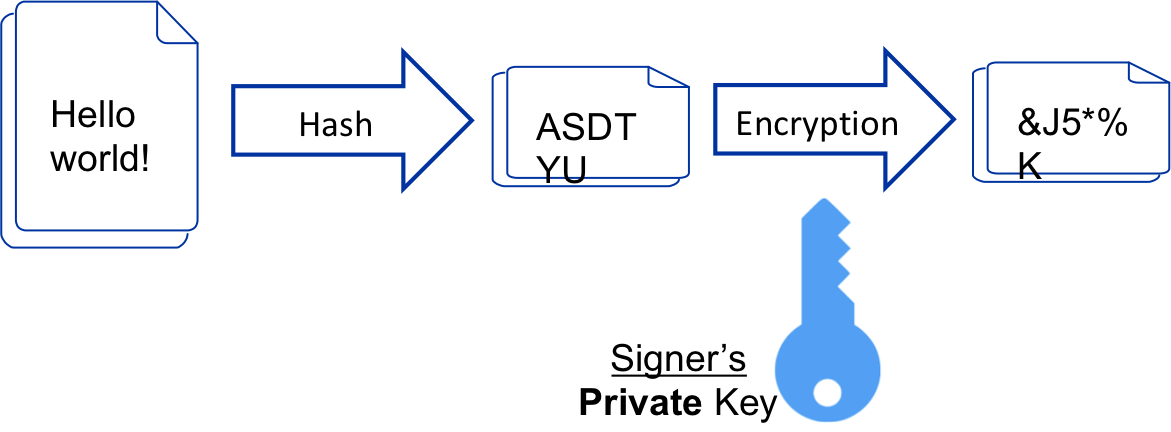
\includegraphics[width=0.9\linewidth]{digital-signature.png}
\end{center}
\end{frame}

\begin{frame}{Certificate Authentication}
Owning a Certificate of Alice does not mean that you are Alice
\begin{itemize}
\item Holding a Certificate does not imply you are authenticated
\item How would you verify that the person who comes to you pretending to be Alice and showing you a certificate of Alice is really Alice ?
\begin{itemize}
\item You have to challenge her!
\item Only the real Alice has the private key that goes in pair with the public key in the certificate.
\end{itemize}
\end{itemize}
\end{frame}

\begin{frame}{{\color{red}Certificate Authentication}}
\begin{center}
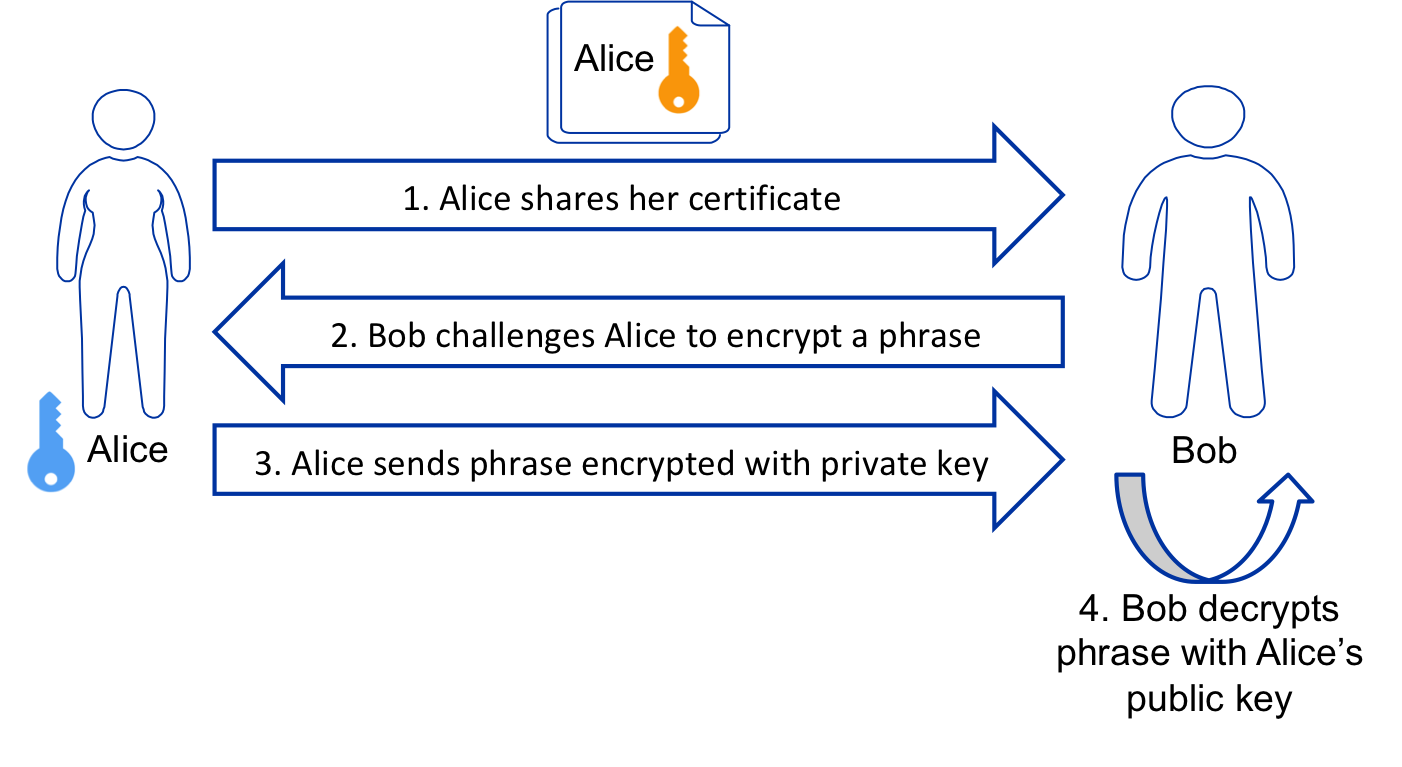
\includegraphics[width=0.9\linewidth]{certificate-verification.png}
\end{center}
\end{frame}

\begin{frame}{Certificates - Summary}
\begin{itemize}
\item Contain a public key, identity information and a signature
\item Certificates are signed by Certificate Authorities who are trusted to validate the certificates
\item Certificates \& private keys together allow asymmetric encryption and authentication
\end{itemize}
\end{frame}

\section{Web Security}
\frame{\sectionpage}

\begin{frame}{Web Security}
All the concepts we just learned are fundamental components of web security! They are used to protect us from attacks, such Eavesdropping or ``Man in the Middle"
\begin{center}
	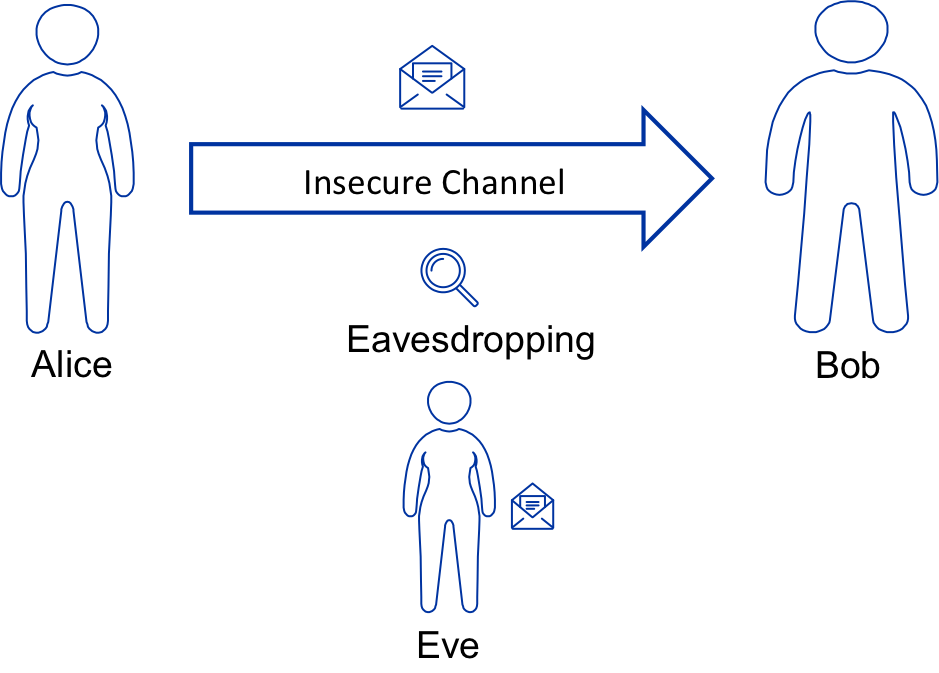
\includegraphics[width=0.5\linewidth]{insecure-channel.png}
\end{center}
\end{frame}

\begin{frame}{{\color{red}HTTPS}}
Hyper-Text Transfer Protocol \textbf{Secure} 
\begin{itemize}
\item HTTPS is HTTP with SSL/TLS (so with encryption)
\item Establishes a secure channel between a client (your web browser) and a server (hosting the web site you're visiting) 
\item Uses asymmetric encryption to authenticate the server 
\item Uses symmetric encryption for the ongoing information exchange
\end{itemize}
\end{frame}

\begin{frame}{{\color{red}HTTPS Handshake}}
\begin{center}
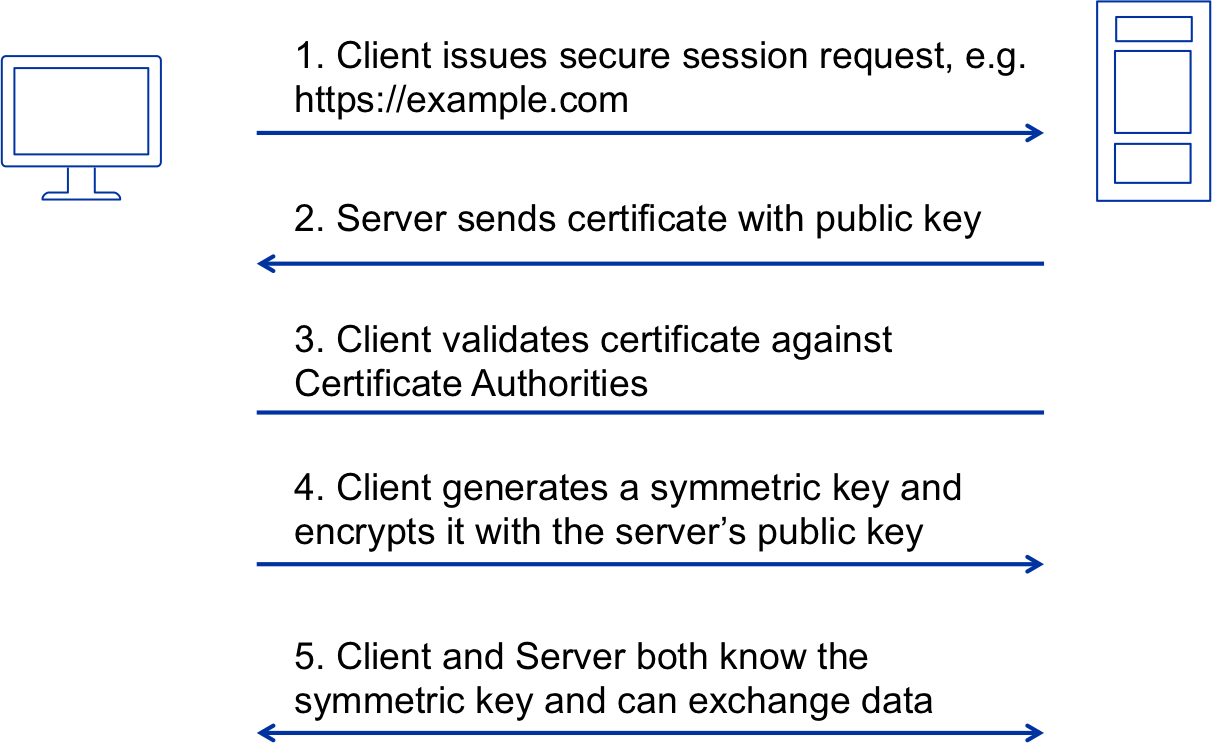
\includegraphics[width=0.8\linewidth]{https-flow.png} 
\end{center}
\end{frame}


\begin{frame}{HTTPS}
How do we know who to trust?
\begin{itemize}
\item Trusted Certificate Authorities issue Certificates to websites, they create the digital signatures (e.g. Comodo, LetsEncrypt)
\item Browsers alert when there is a problem with the certificate, e.g. the description does not match the host name
\end{itemize}
\begin{center}
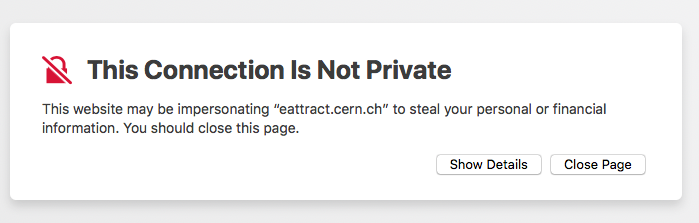
\includegraphics[width=0.5\linewidth]{certificate-error.png}
\end{center}
\end{frame}

\begin{frame}{Web Security DOs and DON'Ts}
\begin{center}
\begin{tabular}{ |p{0.45\linewidth}|p{0.45\linewidth}| }
\hline
\textbf{DOs} & \textbf{DON'Ts} \\ \hline \hline
Respect warnings for invalid certificates & Continue if you're not 100\% sure!\\ \hline
Check that credit cards and passwords are sent over HTTPS & Enter data on forms over HTTP\\ \hline
Verify the checksum of downloaded software & Download software from unverified sources\\ \hline 
\end{tabular}
\end{center}
\end{frame}


\begin{frame}{Web Security - Summary}
\begin{itemize}
\item Certificates and private keys are used to establish authenticated, encrypted channels when you browse the web
\item Asymmetric and symmetric ciphers are used together for HTTPS
\end{itemize}
\end{frame}

\begin{frame}{Questions?}
\begin{itemize}
\item Ask now
\item Find us during the break
\item You are welcome to contact us after the school
\end{itemize}
\end{frame}

\begin{frame}{Credits}
	\begin{itemize}
		\item Michael Davis (CERN IT) for Cypher examples
		\item Remi Mollon (CERN IT) for Encryption examples
        \item Alberto Pace (CERN IT) for Certificate \& Public Key examples
        \item Icons from SlideCarnival
	\end{itemize}
\end{frame}

\backcover

\end{document}